\chapter{Conceptual background}\label{ch:conceptual-background}

In the previous three chapters, I discussed novel data concerning the interaction between partitivity and countability. In particular, I presented linguistic evidence suggesting that singulars and plurals do not differ with respect to the part-whole relation they employ but rather that parts of singularities remain in a particular topological configuration ensuring that the whole constitutes an integrated object, whereas parts of pluralities do not, and thus form a scattered entity. This claim is motivated by two linguistic facts. First, cross-linguistically the same partitive words can appear both in entity and set partitives. Second, the contrast between regular plurals  and Italian irregular plurals reveals a crucial topological distinction between the two. Furthermore, I showed that natural language does not allow for counting arbitrary sums of topologically unrelated parts. Only entities that are conceptualized as constituting continuous objects can be subject to counting. This restriction appears to hold both on the level of wholes and on the subatomic level, as the evidence concerning topology-sensitive partitive words as well as the semantic behavior of multipliers indicate. In other words, quantification in natural language is sensitive to topological relations between parts of entities it operates on.  

In this chapter, I will discuss the conceptual background concerning countability and subatomic quantification I assume here. In particular I will present three claims regarding the relevance of topological notions in nominal semantics, general counting principles, and their significance for subatomic quantification. This informal conceptual framework will motivate the formal account for the core phenomena explored in this study, which I will develop in Chapters \ref{ch:theory-of-parts-and-wholes} and \ref{ch:mereotopological-account-for-subatomic-quantification}. However, before I present in detail the notional core of this study, let us cgonsider a more general cognitive context. Though the linguistic evidence presented so far is compelling and entirely motivates the claims, I believe it is useful to confront it with what we know from psychological research in order to provide supplementary support. 

\section{Psychological evidence}\label{sec:psychological-evidence}

In this section, I will review psychological evidence that demonstrates several factors concerning human cognition that correlate with the linguistic evidence introduced in Chapters \ref{ch:partitives-and-part-whole-structures}, \ref{ch:exploring-topological-sensitivity}, and \ref{ch:multipliers}. First, I will discuss the relevance of how spatial categories such as solidity, shape, and most importantly integrity of entities are conceptualized with respect to the mass/count distinction in grammar. Furthermore, I will consider the significance of the part/whole distinction for language acquisition and review the evidence that humans have simultaneous perception of an object as a whole and as a collection of parts. Finally, I will discuss what cognitive studies tell us on number sense in humans, especially on the relation between integrity and counting in young children. The literature on each topic is abundant. For the sake of brevity, in each case I will only refer to a few representative studies.

\subsection{Object/substance distinction}\label{sec:object-substance-distinction}

I will start with a brief overview of the research in cognitive psychology relating individuation with the difference in perception of solid objects and amorphous substances, which suggests that this distinction is relevant to the phenomenon of countability in natural language. In the past 30 years, convincing evidence has been presented that indicates that the distinction between objects and substances is not merely an alternation based on grammar. Contrary to \citeposst{quine1960word} influential claim that it is language what provides the means for individuation of objects \citep[see also][]{pelletier_schubert1989mass}, it appears that count and mass syntax reflect on how we see entities in the world rather than the other way round. In other words, the research to be discussed here shows that the distinction between objects and substances is not something conventional, formal, or arbitrary imposed by the way a particular language is devised, i.e., a way of speaking so to say. To the contrary, it appears to be a deeply embedded component of human cognition manifesting itself in non-verbal infants at a few months of age and shared with non-human species. 

Multiple experiments demonstrate that children associate count nouns with solid discrete objects at an early age \citep[see, e.g.,][]{landau_smith_jones1988importance,soja_carey_spelke1991ontological,imai_gentner1997crosslinguistic}. The evidence comes from the results of the so-called word extension task, which concerns learning new words by subjects. The procedure is as follows. First, a child is presented with a novel entity and instructed on what it is called. That entity can be either a solid object or a shapeless portion of a substance. Next, two other entities resembling the initial one with respect to different perceptual features are introduced. One would match the already introduced entity in shape, whereas the other would be of the same material. Interestingly, extensive research shows that children extend the name of a novel item to items of the same shape only if the initial entity was a solid discrete object. On the other hand, if they were first presented an amorphous portion of a novel substance, they do not extend its name to items of a similar shape, but rather to objects made out of the same material.

Based on such evidence, \citet{soja_carey_spelke1991ontological} argue that certain ontological commitments are prior to the linguistic mass/count distinction, contrary to \citeauthor{quine1960word}'s claim. Additional support for such a conclusion comes from the fact that the results were replicated in populations using languages with syntax significantly different from English. For instance, \citet{imai_gentner1997crosslinguistic} demonstrate parallel evidence based on the same experimental paradigm using the word extension task in the Japanese speaking environment. Though Japanese lacks a straightforward morpho-syntactic equivalent of the distinction between mass and count nouns present in languages such as English, Japanese speaking children distinguish between objects and substances just as well as their English speaking peers.

A number of studies provide varied and carefully controlled evidence that preverbal children are endowed with certain assumptions concerning the nature of objects \citep[e.g.,][]{carey1985conceptual,spelke1990principles,soja_carey_spelke1991ontological,carey_spelke1996science}. For instance, they expect objects to be bounded and cohesive. The former assumption reflects on an entity having natural boundaries, whereas the latter translates into an anticipation that objects have parts that stick together. Furthermore, objects are expected to move across space as wholes along continuous paths and to retain identity upon collisions with other entities. On the other hand, substances lack any of those properties. An exemplary experimental paradigm is as follows. An infant is introduced either to a solid object, e.g., a teddy bear, or a portion of substance, e.g., clay, displayed in front of them. Next, the entity is covered by a screen and the child sees that a second item is placed behind the screen. Finally, depending on an experimental condition after the screen was removed either there were two items revealed or due to the manipulation by an experimenter only one item could be seen. Interestingly, if the initially introduced entity was a discrete solid object, children reacted with great surprise if after removing the screen they could find only one item. On the other hand, no such reaction was recorded if they were introduced to a portion of a substance at the beginning. The conclusion is that preverbal children appear to know the difference between objects, pluralities thereof, and substances. They expect that if one adds a teddy bear to a teddy bear, the result should be two teddy bears, whereas if one combines clay with clay, one does not get a plurality of clay. Since similar results were also found in non-human primates (see, e.g., \citealt{hauser_carey2003spontaneous,hauser_spaulding2006wild} on rhesus monkeys), it seems plausible to assume that this property of human cognition has some evolutionary history. I will come back to the issue of number in \sectref{sec:number-sense}.

However, though the difference between discrete solid objects and amorphous substances has a significant status in the cognitive and linguistic development of children, it turns out that the correlation between this distinction and mass/count syntax is imperfect. A corpus study on toddler vocabulary pursued by \citet{samuelson_smith1999early} shows a significant asymmetry between particular syntactic categories. Specifically, while the large majority of nouns that English speaking children learn early are count nouns (74\% of the vocabulary), only a small portion involves mass nouns (10\% of the vocabulary). There is also a third class of expressions that is considered ambiguous between count and mass (16\% of the vocabulary). The results of the examination in order to find out whether the object/substance distinction correlates with the mass/count distinction are somewhat surprising. In general, a correspondence between solid objects and count nouns, on the one hand, and non-solid entities, on the other, was in fact observed. However, it was imperfect and \citeauthor{samuelson_smith1999early} recognized a number of interesting mismatches. Surprisingly, while solidity and shape turn out to be good predictors of count nouns, mass nouns appear to be less correlated with non-solidity and shapelessness.\footnote{Notice that probably the main reason explaining this result is the existence of the category of object mass nouns such as \textit{furniture} and \textit{kitchenware}.}

Yet another strand of research provides support for the findings discussed above. In particular, \citet{prasada_ferenz_haskell2002conceiving} demonstrate that categorization of a noun as countable or uncountable does not reduce to establishing an immutable ontological distinction between an object and a substance. Rather, it seems that speakers of languages such as English categorize nouns in terms of countability based on whether they construe entities they refer to as objects or as substances. A series of experiments utilizing novel vocabulary tasks show that a novel item that has an irregular shape is less probable to be referred to by a novel count noun when contrasted with entities of a regular shape. However, the same item is significantly more probable to be considered countable when displayed among other similar entities having such an irregular shape. This means that it is not the case that some objective properties of things influence the way grammar is directly. Instead, the mass/count distinction appears to reflect how humans conceptualize entities in the world.

To conclude, the psychological research reviewed in this section indicates that contrary to \citeauthor{quine1960word}'s claim, human beings apparently do have certain ontological commitments prior to acquiring the syntax of a particular language. Specifically, the way children are biased towards perceiving objects as opposed to substances correlates with the mass/count distinction in grammar. However, this correspondence is not of a one-to-one  type and there are well-known cases of mismatches. Yet, it is crucial that the distinction in grammar is not due to different ontological categories in some objective sense, but rather it reflects on how entities in the world are conceptualized. In the next section, I will discuss the relevance of part-whole structures in the process of language acquisition. In particular, I will briefly review how a certain bias concerning what it means to be a whole guides children in how they learn lexical meanings of nouns. 

\subsection{Whole object assumption}\label{sec:whole-object-assumption}

Since at least the early 1990's, language acquisition studies have shown that vocabulary development is constrained by certain mechanisms that govern it in order to ensure its effectiveness. In particular, children are guided by a number of word learning biases i.e., endowed assumptions that allow us to eliminate unlikely alternatives in order to efficiently process and learn new lexical meanings \citep[see, e.g.,][]{markman1990constraints,hollich_golinkoff_hirsh-pasek2007young,hansen_markman2009children}. Such assumptions begin to manifest around the age of 18 months when rapid expansion of a child's vocabulary starts. They are crucial in deciding what the reference of a new noun is, e.g., what aspect of an object it designates, as well as in solving the problem of indeterminacy. One of the word learning biases that will be of special interest to us here is the so-called whole object assumption \citep{markman1990constraints}. 

The whole object assumption allows children to constrain the meaning of novel words by guaranteeing that a child relates a new noun with an object in its entirety rather than with some arbitrary part or property of that object \citep{markman1990constraints}. For instance, if an adult points to an item and labels it, e.g., by uttering \textit{a doll}, a child assumes that the noun \textit{doll} is meant to refer to the whole object and not to its part or its certain characteristic. Though in principle the adult's verbal behavior might have been interpreted as referring to the doll's head, leg, dress, color, or size, children intuitively rule out such possibilities and associate the label with the whole item.\footnote{See \citet{quine1960word} for a related problem of the inscrutability of reference.} This bias holds even in situations where an object's color or a certain dynamic activity are made salient to a child \citep{hansen_markman2009children}.

Though the original research regarded 18-month-year old children and older, later studies have demonstrated that in fact infants can associate nouns with whole objects already at the age of 12 months \citep{hollich_golinkoff_hirsh-pasek2007young}. Crucially, the effect was attested despite the fact that test items could be viewed as two separate objects and even when a certain part of an item was made salient. Interestingly, similar results were obtained in experiments where participants were adult. Hence, the mechanism appears to be deeply embedded. Its relevance lies in that it enables children to determine which of the numerous logically possible meanings a word could have is actually the correct one.

In this section, we saw that children distinguish intuitively between parts and wholes. In the process of language acquisition, when exposed to a novel noun, they do not attribute its meaning to a part of an object it refers to but rather immediately assume it is true of a whole thing. The whole object assumption has often been related to the findings concerning infants' perception of objects discussed in the previous section. It has been hypothesized that the constraint in question reflects the non-linguistic status of objects \citep{hollich_golinkoff_hirsh-pasek2007young}. This might suggest that from the perspective of a child the fact that wholes involve parts is somewhat discriminated. However, the evidence is much more complex. In the next section, I will provide a brief overview of the study of part-whole perception in children.

\subsection{Part-whole perception}\label{sec:part-whole-perception}

It is a cognitive fact that we often conceive of entities as being made up of smaller entities related to each other in a particular manner. Experimental evidence shows that humans have two simultaneous perceptions concerning part-whole structures of entities \citep[e.g.,][]{witkin1950individual,meili-dworetzki1956development}. On the one hand, we possess the ability to discriminate parts from a whole, i.e., decompose an entire object into distinct elements making it up. On the other hand, we are able to integrate the total sum of the parts into a complete whole. This phenomenon is usually referred to as part-whole perception and it is standardly attributed to the ability of an individual to decenter, i.e., to shift attention from parts to the whole or vice versa \citep[see][]{piaget_morf1958isomorphismes}.

Though adults in general show part-whole perception, it has been subject to controversy in the psychological literature at what age it emerges. In the early Piagetian studies, the experimental results suggested that this ability is absent in young children \citep{elkind_koegler_go1964studies}. In a typical experiment, a child was presented a drawing of a whole consisting of parts that were independent objects in their own right, e.g., a person made out of fruits as in \figref{fig:part-whole-perception}, and was instructed verbally to report what they see. 

\begin{figure}[h!]
\centering
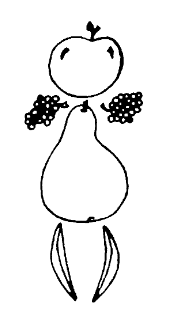
\includegraphics[scale=0.3]{figures/fruitman.png}
\captionof{figure}{Part-whole perception \citep{elkind_koegler_go1964studies}}\label{fig:part-whole-perception}
\end{figure}

According to \citeauthor{elkind_koegler_go1964studies}, children report that they perceive simultaneously a whole and parts attributed to the same form, e.g. both a man and fruits, only at the age of 8. Before that age, subjects failed in complete decentration with 5-to-6-year-olds showing complete centration, i.e., they reported that they saw only parts, e.g., fruits but not a person, and older children gradually improved. However, later studies suggest that part-whole perception develops much earlier. For instance, \citet{kimchi1993basic} provides evidence that 5-year-old children show sensitivity to parts and to part-whole relations and that this sensitivity improves with age. Even more interestingly, \citet{boisvert_standing_moller1999successful} show that 3-year-olds demonstrate good performance in part-whole perception tasks using multiple-choice tests instead of Piagetian verbal tasks used in earlier studies. Finally, \citeposst{quinn_burke_rush1993part} results indicate that 3-month-old infants can group elements of visual pattern information into larger perceptual units based on lightness similarity in a way that suggests at least some component of part-whole perception.

I interpret the experimental results presented above as suggesting that human cognition is devised to be sensitive to part-whole structures since even very young individuals can decompose a whole into pieces by discriminating its parts as well as represent individual elements as making up an integrated collection that is a whole. Since these two perceptions are simultaneous, one could expect that we intuitively categorize entities as certain configurations of smaller things that despite their often complex inner structure are singular objects. At the same time, parts of such objects remain cognitively salient and if required, can be easily accessed. If the conclusions from the experiments reported above are on the right track, this property of the human mind appears to be either innate or at least to emerge at an early stage of cognitive development.

\subsection{Number sense}\label{sec:number-sense}

The final piece of cognitive evidence to be discussed here concerns human number sense, i.e., an intuitive understanding of what numbers mean and how they can be affected by various operations (see, e.g., \citealt{dehaene1997number} for an overview). This mental mechanism allows for a special type of sensory perception through which the cardinality of a given set of entities can be perceived with similar ease as their size, color, shape, or position and as such provides the basis for various forms of calculation. In humans, number sense is based on two different cognitive systems, specifically the approximate number system (ANS) and the object tracking system (OTS) \citep[see, e.g.,][]{hyde2011two}. The ANS is a cognitive system supporting the imprecise estimation of the numerical magnitude of a collection of objects without relying on symbolic representations (see, e.g., \citealt{feigenson_et-al2004core,nieder_dehaene2009representation} for an overview). It manifests already in infants and gets more developed with age \citep{cantlon_et-al2006functional}. In contrast, the OTS is the mental ability to independently track up to 4 entities without counting by means of parallel individuation (see, e.g., \citealt{carey1998knowledge,carey2009origin} for an overview). Though the acquisition of abstract number concepts, even for low numbers, appears to require more than only the ANS and the OTS, both capacities seem to support this process (e.g., \citealt{hyde2011two}; but see \citealt{piazza2010neurocognitive} for arguments for the crucial role of the ANS rather than the OTS).

It appears that there is evidence indicating that humans are at least to some extent predisposed to develop certain numerical abilities such as the concept of exact number and simple arithmetic based on their number sense. For instance, \citet{gelman_gallistel1978child} argue that children are endowed with innate principles of counting and have intuitive understanding of the cardinality of a set of entities and its conservation under changes that do not affect quantity. It seems that a lot of knowledge concerning how to put objects in a one-to-one correspondence with numbers is intuitively understood by children though it is never taught or formulated in an explicit way. In particular, when learning to count children are not taught that each entity must be counted once and only once, or that one number cannot be associated with more than one entity, but this principle is taken for granted. Moreover, children know intuitively that number words are supposed to be recited in a fixed order and that the last numeral represents the cardinality of the whole enumerated set. According to this view, innate knowledge regarding counting principles precedes and facilitates the acquisition of that part of the lexicon that includes number words and guides its application in a particular situation of counting.\footnote{However, see \citet{fuson1988springer} for an opposing view claiming that children learn counting by imitation. For instance, \citeauthor{fuson1988springer} argues that children recite strings such as \textit{onetwothreefourfive}\dots {} as uninterrupted sequences and only later on they segment them in order to delimitate numerals, learn to extend them to larger values and to apply them to particular situations.}

The above introduced hypothesis seems to be corroborated by further experimental evidence that suggests that at the age of 2.5 years children understand that counting is an abstract procedure that can be applied to different kinds of objects including concrete entities as well as events \citep{wynn1990children}. 3.5-year-olds know that the order in which they recite numerals is crucial, whereas the order of pointing at counted items is irrelevant as long as each item is counted and no one item is counted twice. Furthermore, children are able to indicate and correct subtle errors that result from violations of basic counting principles such as reciting numerals out of order, counting the same object twice, or omitting an item while counting \citep{gelman_meck1983preschoolers,gelman_meck_merkin1986young}. By the age of 4 years, children show that they have already mastered the basics of counting and that they can generalize the procedure to novel situations. Older children often spontaneously reinvent arithmetic developing new strategies for calculating that best fit for a particular problem \citep[p. 119]{dehaene1997number}.

However, probably the most intriguing finding from the perspective of the interest of this study is a tight link between spatial integrity and numerical information observed in young children. Specifically, \citet{shipley_shepperson1990countable} provide a particularly striking demonstration of the relevance of objects understood as integrated discrete physical entities for the cognition of 3-to-4-year-olds. In the experiment, children were presented sets of items and instructed specifically what they were supposed to count. For instance, an array of forks with one item broken in two pieces as illustrated in  \figref{fig:relevance-of-integrity-in-counting} was displayed in front of a child who was then asked to count the forks. 

\begin{figure}[h!]
\centering
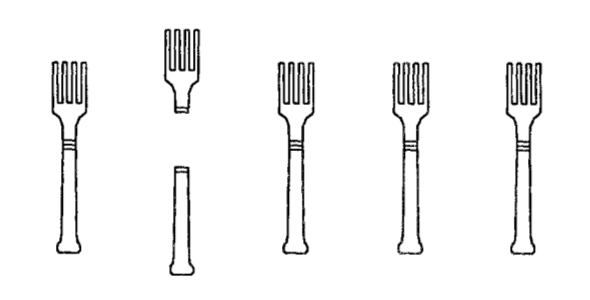
\includegraphics[scale=0.4]{figures/forks.png}
\captionof{figure}{Relevance of integrity in counting (\citealt[p. 60]{dehaene1997number}; adapted from \citealt{shipley_shepperson1990countable})}\label{fig:relevance-of-integrity-in-counting}
\end{figure}

Unlike adults and older children, children between 3 and 4 years of age did not answer that there are five forks, but rather that there six of them, i.e., they counted each detached part of a fork as a separate entity. Similarly, when instructed to count kinds, e.g., different kinds of animals, or properties, e.g. different colors, in a setup where each kind or property was exemplified by a number of distinct discrete items, children included each separate object in their count.

The results demonstrate that the canonical countable entity for a young child is a discrete physical object that comes in a single piece. The role of spatial integrity is crucial in determining what counts as one and this bias precedes the process of learning how to count. In other words, at an early stage of development of arithmetic abilities young children simply cannot avoid counting each discrete integral object as one unit. It is very likely that the assumption that number is a property of sets consisting of discrete spatially contiguous objects is a deeply embedded principle that facilitates mastery of counting.\largerpage[2]

The findings of \citeauthor{shipley_shepperson1990countable} were further confirmed for other forms of linguistic quantification in experiments based on quantity judgment tasks involving comparative constructions and pluralization \citep{melgoza_pogue_barner2008broken}. In particular, when presented an object divided into three parts, e.g., a broken fork, on the one hand, and two whole objects, e.g., two integral forks, on the other, 4-year-old children judged the former to be more objects than the latter. Furthermore, in an elicitation task children often labeled broken objects using plural morphology. For instance, a phrase \textit{some forks} was used to refer to three separated pieces of a broken fork. The results presented by \citeauthor{melgoza_pogue_barner2008broken} not only confirm the findings of \citeauthor{shipley_shepperson1990countable} but also indicate the existence of a spatial bias for many forms of quantification in natural language. In all tested cases, the spatial criterion of integrity was preferred over other factors in order to establish what counts as one. In other words, when children quantify sets, they seem to define individual set members in terms of spatial contiguity in the first place. I take these results to be  evidence suggesting that countability as a property of sets of discrete separate entities is a deeply embedded principle. Though as we know from every-day life experience adults can develop a mechanism to retrieve the original part-whole structure of counted entities, e.g., reconstruct a whole fork by combining separate pieces in thought, I hypothesize that the underlying quantificational procedure is based on a principle relating numbers with things that are conceptualized as coming in one piece.{\interfootnotelinepenalty=10000\footnote{Admittedly, one can also count concrete entities such as functional units that do not seem to be integrated in a topological sense. For instance, a pestle and mortar can count as a single piece of kitchenware \citep{sutton_filip2016counting}. Nevertheless, I argue that in such cases the notion of integrity still applies, though it is not physical integrity but rather functional units are conceptually integrated in the sense that they are united under some functional role \citep[see][]{grimm_levin2017artifacts}. I will come back to this issue in \sectref{sec:functional-units}.\label{fn:artifacts}}} However, before I conclude, I will briefly discuss how human quantification differs from number sense in other animals.

Massive evidence indicates that number sense is not exclusive to human mind. Well-established research in etiology shows that apprehension, comparison, and even approximate addition of quantities is also present in animals (see, e.g., \citealt[pp. 13--40]{davis_perusse1988numerical,gallistel1989animal,dehaene1997number} for overview). The most well-known evidence concerns the ability to represent and discriminate quantities of relative sizes in primates \citep[e.g.,][]{woodruff_premack1981primative,matsuzawa1985use,rumbaugh_et-al1987summation,washburn_rumbaugh1991ordinal,boysen_et-al1996quantity}, but it is also found in other mammals such as dolphins \citep{mitchell_et-al1985discriminative}, cats \citep{thompson_et-al1970number}, and rats \citep{capaldi_miller1988counting}, as well as birds \citep{pepperberg1987evidence} and even fish \citep{agrillo_et-al2012evidence}. Furthermore, recent studies in botanics suggest that there are reasons to also assume plant arithmetic \citep{bohm_et-al2016venus}. The evidence indicates either that number sense is an evolutionary ancient part of cognition or that there were multiple convergent evolution events. In any case, it is a widespread phenomenon shared by a wide range of species.

However, despite the large body of evidence indicating that many non-human animals have the approximate number system, their number sense seems to differ significantly from that of humans. Though there are well-documented cases of approximate quantification in animals, no case of symbolic addition is known in any species other than the chimpanzee, and there only after long training dedicated to learning a small set of digits and with frequent errors in computation \citep[p. 39]{dehaene1997number}. On the other hand, young children spontaneously count on their fingers, often up to 10 before the age of three and acquire the syntax of complex numerals with ease. Thus, the more lax concept of numerosity is often used with respect to animal quantification in order to distinguish it from the symbolic and verbal representation of number in humans. To conclude, though some forms of quantification appear to be frequent in the animal kingdom, they seem to differ significantly from what humans do when they count. While non-human animals estimate quantities on a regular basis, it seems that the ability to establish a one-to-one correspondence between an object and a discrete symbol which allows for computation of the exact number of entities in a given set is an extremely rare property among species. 

It seems that counting as performed by humans is a quite unique ability which associates discrete entities with abstract representations of number. I hypothesize that the core  mechanism underlying all counting manifests in early childhood and concerns establishing a one-to-one correspondence between integral physical objects that come in one piece and integers. In other words, I assume that the topological notion of spatial integrity is the basis for what counts as one, and only later humans develop ways of abstracting away from this principle, e.g., by extending it to quantification over abstract entities such as kinds and properties, or by being able to retrieve the original connection between detached parts. In the following sections, I will attempt to relate the linguistic evidence presented in Chapters \ref{ch:partitives-and-part-whole-structures}, \ref{ch:exploring-topological-sensitivity}, and \ref{ch:multipliers} with the conclusions of cognitive psychology in order to develop the three main claims of this study that will serve as a conceptual background for the formal account for subatomic quantification in natural language, to be developed in Chapters \ref{ch:theory-of-parts-and-wholes} and \ref{ch:mereotopological-account-for-subatomic-quantification}.

\section{The three claims}\label{sec:the-three-claims}

I have already presented a broad range of data demonstrating both the relevance of subatomic structures in natural language and the important role that the way entities including parts of a whole are spatially related to each other plays with respect to quantification. Furthermore, in the previous section I reviewed additional psychological evidence suggesting that these issues are deeply embedded in human cognition. Now is the time to discuss in detail what I believe to be the conceptual core of this study, namely the three claims I make with respect to the interaction between parthood, topology, and quantification in natural language. I will start with postulating that natural language semantics is sensitive to topological relations holding between elements within part-whole structures designated by nominal expressions. Next, I will posit a set of general counting principles, including constraints concerning non-overlap, maximality, and integrity of counted things. Finally, I will postulate that the very same universal mechanism applies irrespective of whether one quantifies over entire entities or over parts of a whole.

\subsection{Relevance of topological notions with respect to part-whole structures}\label{sec:relevance-of-topological-notions-with-respect-to-part-whole-structures}

It is well-known that topological notions play an important role in natural language. The existence of locative expressions involving prepositions such as \textit{inside}, \textit{near}, \textit{under}, \textit{between}, and \textit{far} shows that relations concerning how we conceptualize position and space are deeply rooted in grammar. Arguably, they constitute universal components of human cognition and natural language semantics. Though the research on locative PPs is well-established and contributed to our understanding what means language uses to encode information regarding location of objects with respect to each other \citep[e.g.,][]{clark1973space,herskovits1985semantics,zwarts_winter1997semantic,kracht2002semantics}, the question concerning spatial constitution of entities remained somewhat elusive in the study of meaning. One line of argumentation justifying why those kinds of issues should remain unaddressed is that they simply stem from every-day world knowledge, and thus, as extra-linguistic factors, are not supposed to be incorporated into semantic theory. For instance, \citet{schwarzschild1996pluralities} famously argues that the fact that \ref{ex:bill-texas} entails \ref{ex:brain-texas} has nothing to do with referential properties of the subject DPs in both sentences. Rather, the inference simply results from facts concerning what we know about where brains are located. 

\ex. English \citep[p. 187]{schwarzschild1996pluralities}\label{ex:bill-brain-texas}
\a. Bill is in Texas.\label{ex:bill-texas}
\b. Bill's brain is in Texas.\label{ex:brain-texas}

\citeauthor{schwarzschild1996pluralities} might seem right for examples such as \ref{ex:bill-brain-texas}. However, in previous chapters of this study we saw that there are a number of natural language expressions that are sensitive to topological properties of part-whole structures corresponding to their referents. My view is that if we want to account for the meaning of nouns in its entire complexity, topology-related phenomena deserve serious consideration.

It has been acknowledged for a long time that nominal semantics differentiates between count singulars referring to integrated objects, on the one hand, and mass terms and plurals denoting scattered entities and arbitrary sums of individuals, respectively, on the other. As we saw in \sectref{sec:object-substance-distinction}, there are good reasons to assume that this contrast correlates with some fundamental properties of human cognition. Soon, we will see that the distinction can be captured in terms of how parts constituting a whole are spatially arranged. However, before I even start considering how to develop a proper account, it is crucial to realize that the extent to which topology plays a role in part-whole structures associated with referents of nominals is highly underestimated, if not neglected, in the contemporary mainstream research on pluralities and countability. One of the important empirical contributions of this study is about compensating this deficit. 

The data presented in Chapter \ref{ch:partitives-and-part-whole-structures} and \ref{ch:exploring-topological-sensitivity} show that certain classes of nouns encode certain types of spatial configurations of entities making up a whole. In particular, at least some Italian irregular plurals discussed in \sectref{sec:italian-irregular-plurals} denote integrated pluralities, i.e., sums of individuals that form cohesive wholes. On the other hand, different types of topology-sensitive partitive words explored in \sectref{sec:continuous-discontinuous-parts} and \sectref{sec:more-topology-sensitive-partitive-words} involve reference to continuous parts whereas extensions of their topology-neutral counterparts comprise also discontinuous portions of a whole. Though the evidence explored in this study emphasizes specifically the role of integrity in subatomic quantification, recent research on different types of collective nouns and mass terms points to a similar conclusion regarding the relevance of topology in nominal semantics on independent grounds. In particular, \citet{grimm2012number} proposes that a subset of mass nouns that denote aggregates of granular objects, hence granular mass terms like \textit{rice} and \textit{gravel}, involve reference to clustered individuals, i.e., bundled entities transitively connected to each other. In a similar vein, \citet{henderson2017swarms} argues that swarm nouns such as \textit{grove}, \textit{horde}, and \textit{swarm} denote large pluralities whose constituents remain in proximity within a certain spatial configuration. Moreover, \citet{grimm_docekal-toappear-counting} and \citet{wagiel-toappear-slavic} discuss a particular class of Slavic derived mass nouns, such as Czech \textit{list} `leaf' $\sim$ \textit{listí} `foliage', that refer to collections of singular entities that are easily distinguishable yet conceptualized as aggregates.\footnote{For experimental investigation into the meaning of such expressions in Czech and Polish, see \citet{docekal_wagiel2018decomposing}.} Finally, as proposed by \citet{grimm2012number}, referents of concrete count nouns can be viewed as entities whose part-whole structure is constrained in such a way that it forms an integrated object in its own right.

The psychological evidence discussed in \sectref{sec:psychological-evidence} emphasizes the role of spatial integrity of objects, on the one hand, and our ability to simultaneously perceive individual parts of such cohesive wholes as entities in their own right, on the other. Given the amount of linguistic evidence supplemented with findings concerning human cognition, I argue that semantic theory needs to accommodate those facts. In other words, my first claim is as follows. There is more to the meaning of common nouns than usually assumed, and without a proper approach incorporating the insights concerning the role of topological notions in part-whole structures many phenomena will be left unexplained or even unnoticed. I posit that a good starting point is to try to capture the difference between count singulars, regular plurals, and mass nouns in terms of different topological relations encoded within corresponding part-whole structures. Specifically, count singulars refer to entities that constitute integrated wholes whose parts stick together, rather than mere collections of spatially unrelated portions of matter. On the other hand, plural nouns denote arbitrary sums of such individuals, i.e., they require their parts to be constrained by spatial integrity but impose no topological restrictions on configurations in which they appear. Finally, a proper treatment of mass terms should account for the fact that their prototypical referents are scattered unbounded entities. An additional advantage of such a novel perspective is that it suggests that different part-whole structures do not emerge due to distinct parthood relations. Instead, it seems that different part-whole structures arise as a result of the interaction between one unified parthood relation with distinct topological notions. In the next section, I will posit that the postulated view on what it means to be a whole can shed new light on countability.

\subsection{General counting principles}\label{sec:general-counting-principles}

In general, I follow a well-established linguistic tradition assuming that the mass\slash count distinction corresponds to a contrast concerning how different types of entities are conceptualized \citep[e.g.,][]{wierzbicka1988semantics,chierchia1998plurality,chierchia1998reference,chierchia2010mass,chierchia2015universal,grimm2012number}. As we saw in \sectref{sec:psychological-evidence}, a substantive body of research in cognitive psychology provides evidence that human beings categorize stable bounded things that preserve shape differently than amorphous substances. The former are considered delimited objects whose spatial identity can be tracked easily throughout time, whereas the latter are perceived merely as unindividuated portions of matter. On the other hand, there appears to be rich intuitive knowledge concerning what counting is, which seems to be part of human cognitive endowment. The exact nature of how cognitive facts relate to natural language semantics and grammar, i.e., the structure and meaning of certain syntactic constructions,  might not be straightforward. Therefore, the view that I propose here is most probably a simplified account. Nevertheless, I believe that it reveals what I argue is an advantageous perspective on what it means to be countable. 

Usually in the study of countability, at some point when it comes to defining what counting is something like `counting is quantification over what counts as one' is stated. Often, `what counts as one' is understood in terms of atomicity. In particular, an atom in a technical sense is an object that has no proper parts. Though at first blush this notion seems rather counterintuitive (see \citealt{champollion2010parts,champollion2017parts} for discussion), it has been very influential in the research on countability.\footnote{I will come back to this issue in \sectref{sec:doing-without-atoms}.} To the extent that counting is often implicitly assumed to be simply quantification over atoms, spelling out the exact nature of the mechanism is rarely provided. In this section, I will attempt to elaborate a bit more on what counting is and how it differs from other forms of quantification. For this purpose, I will consider three conditions entities need to satisfy in order to be able to be put in a one-to-one correspondence with natural numbers based on what we know what humans do when they count. In particular, I will propose three general counting principles that will allow us to better understand countability in a more general manner. Though the proposed mechanism, as described below, is intended to apply only to concrete entities and will require certain additional assumptions with respect to (at least some) artifacts and functional units, I believe that in principle it can be generalized to cover also more abstract domains. As we will soon see, this novel perspective will also prove of great significance with respect to subatomic quantification.

Counting is usually understood as establishing a one-to-one correspondence between what is being counted and natural numbers. This kind of association is necessary to determine the cardinality of a particular set of entities. Though there are a number of aspects of counting, as well as many morphologically distinct numerical expressions dedicated to particular quantificational purposes, including cardinal numerals, ordinals, fractions, percentage expressions, nominals such as \textit{dozen}, approximators like \textit{hundreds}, and numerical adverbials, e.g., \textit{twice}, it is usually assumed that at the end their interpretation is based on number \citep[see][]{rothstein2017semantics}.\footnote{Notice also that both complex numerical expressions are necessary if a language is to be able to enumerate the infinite series of numbers since in order to do so it requires a recursive system \citep[pp. 12--13]{rothstein2017semantics}.} In particular, different types of numerical expressions appear to represent enumerations of different types of sets, e.g., sets of entities as opposed to sets of events.

However, though the definition introduced above involves a significant component of counting, it is incomplete, and thus fails to capture what counting really is and how it differs from other quantificational operations such as measuring. As we will soon see, there are a number of situations where despite successfully establishing a one-to-one correspondence between entities and numbers we would intuitively reject a particular enumeration as counting. Therefore, a more specific characterization is required. In particular, I take counting to be a quantificational operation that is governed by three general principles restricting what kind of object can be assigned a number. I will refer to those constraints as the principle of \textsc{non-overlap}, \textsc{maximality}, and \textsc{integrity}. It is not unlikely that their knowledge is inherent, and thus when talking about counting, their existence is taken for granted. That is precisely why I believe it might be useful to formulate them explicitly in order to get a better understanding of the phenomenon of countability. 

The principle of non-overlap ensures that things that count as one must not overlap, i.e., do not share a part \citep[see][]{landman2011count,landman2016iceberg}. Guaranteeing disjointness of units of counting is necessary to avoid the possibility of an entity being counted twice. For instance, assume portions of matter $a$, $b$, $c$, and $d$ arranged in such a way that $c$ overlaps with both $a$ and $b$, specifically $c = a\sqcup b$. Now, one could imagine an operation that would assign numbers to all $a$, $b$, $c$, and $d$. Summing them up would yield number 4 but this result is incorrect if one wanted to count how many portions of matter there are. The reason is that $c$ is not disjoint from $a$ and $b$, and thus should not be associated with a number.\footnote{Notice that this effect can also be captured by ensuring that the counted set is quantized \citep{krifka1989nominal}, which is a weaker notion than non-overlap. However, I prefer the notion of non-overlap in order to provide a unified system that explains the difference between counting and measuring, see \sectref{sec:counting-vs-measuring}.} To put it differently, when counting it is disallowed to count a thing two times.  

Though prototypical count nouns such as \textit{cat} and \textit{apple} denote sets of mutually disjoint entities, i.e., individual apples have no part in common and the same applies to individual cats, mass overlap, i.e., overlap between material parts of different entities is not inconceivable. For instance, it is possible to imagine three entities conceptualized as distinct objects $a$, $b$, and $c$ such that $a$ consists of three parts $d$, $e$ and $f$ ($a = d\sqcup e \sqcup f$), $b$ consists and of $f$, $g$, and $h$ ($b = f\sqcup g \sqcup h$), and $c$ consists of $h$, $i$, and $j$ ($c = h\sqcup i \sqcup j$). Or to use \citeposst{landman2011count} example, two hands of a certain person and their ten fingers are countable objects despite the fact that each hand shares material parts with its five fingers. Nonetheless, it seems that the way counting operates is that if we can count entities simultaneously as one, in that very counting situation we perceive them as disjoint objects, and any potential mass overlap is ignored. In other words, entities in the count domain are conceptualized as if they do not overlap, irrespective of what the exact structure of the corresponding things in the external world looks like. Given the human part-whole perception discussed in \sectref{sec:part-whole-perception}, I suggest that an ability to perceive objects this way is likely. 

Furthermore, \citet{rothstein2010counting} shows that though a non-prototypical count noun such as \textit{fence} might denote overlapping entities, in a particular situation its denotation is restricted to eliminate overlap. For instance, consider rectangular fence structure $a$ consisting of four fences $b$, $c$, $d$, and $e$ constructed by four different persons; thus, $a = b\sqcup c\sqcup d\sqcup e$. Depending on the context, we could count it as one fence ($a$) or as four fences ($b$, $c$, $d$, and $e$), but never as five fences in a single counting situation. In addition, \citet{krifka2009counting} discusses cases in which one counts configurations such as outfits, e.g., outfits $a$ and $b$ may both consist of pants $c$ and shirts $d$ and $e$, respectively. Such configurations can be conceptualized as distinct things despite the overlap. Crucially, however, such entities cannot exist simultaneously in one and the same situation. Rather, each of the possible combinations can come into being only if the other one is not chosen. Therefore, I conclude that counting typically requires non-overlap while in some non-typical cases it makes overlap irrelevant for how objects are conceptualized. 

The second principle concerns maximality understood in terms of mereological exhaustivity. It states that counting requires that what is associated with a number needs to be a maximal entity of which a certain property holds in a given counting situation. In other words, objects need to be counted in their entirety, i.e., all relevant parts of a thing need to be put in correspondence with a particular number and it is disallowed to leave some of them out. To illustrate this, let us consider a situation where there are three distinct cuboid entities $a$, $b$, and $c$ such that $c$ consists of two non-overlapping parts $d$ and $e$ ($c = d\sqcup e$), as depicted in \figref{fig:counting-and-maximality}. 

\begin{figure}[h!]
\centering
\begin{tikzpicture}
  \draw (0,0) -- (2.5,0) -- (2.5,2) -- (0,2) -- (0,0);
  \draw (3.5,0) -- (5,0) -- (5,2) -- (3.5,2) -- (3.5,0);
  \draw (6,0) -- (9,0) -- (9,2) -- (6,2) -- (6,0);
  \draw[dashed] (7.25,0) -- (7.25,2);
  \node at (1.25,1) {$a$};
  \node at (4.25,1) {$b$};
  \node[fill=white] at (7.5,1) {$c$};
  \node at (6.625,0.5) {$d$};
  \node at (8.125,0.5) {$e$};
\end{tikzpicture}
\caption{Counting and maximality}
\label{fig:counting-and-maximality}
\end{figure}

Now, let us assume that we are counting cuboids and that that is all what the context specifies. We can then imagine a quantificational operation that satisfies the non-overlap constraint but is not restricted by the principle of maximality. In this particular counting situation, when applied to the set of things in question, it might very well yield 4 since $a$, $b$, $d$, and $e$ are disjoint cuboid entities, whereas $c$ shares a part with both $d$ and $e$. However, such an operation would not be of great help if one wanted to know how many cuboids there are since it fails to differentiate between wholes and their parts. Likewise, if one asked for two cuboids and got object $c$ as a result of the request, they surely would not be satisfied.

Of course, situations such as the one described above are rare. Typically, the combination of the predicate and the context provide enough information to specify a counting situation unambiguously, so that there is little doubt regarding what counts as one. For instance, let us suppose that the rectangles in \figref{fig:counting-and-maximality} represent buildings such that $a$ and $b$ are each a detached house, whereas $c$ is a building consisting of two semi-detached houses $d$ and $e$. If one wanted to know the number of houses, the answer would be four ($a$, $b$, $d$, and $e$; assuming that $c$ is not in the extension of the predicate \textit{house}). If, on the other hand, we were counting buildings, then the answer would be three ($a$, $b$, and $c$). Therefore, it might seem that in this particular case the principle of maximality is not playing a role. However, it is possible to find examples which demonstrate that the principle of maximality does apply after the enforcement of contextual disjointness. 

In order to show the relevance of the interaction between maximality and context, let us consider the configuration in \figref{fig:counting-maximality-and-context}, depicting a scenario in the spirit of \citet{rothstein2010counting}. 

\begin{figure}
\centering
\begin{tikzpicture}
  \draw (-2.0,1.0) -- (-2.0,2.0) -- (-1.0,2.0) -- (-1.0,1.0) -- (-2.0,1.0);
  \draw (0,0) -- (0,3) -- (3,3) -- (3,0) -- (0,0);
  \draw[dashed] (2.75,1.5) -- (3.25,1.5);
  \draw[pattern=south east lines,pattern color=gray!25] (1.0,1.0) -- (1.0,2.0) -- (2.0,2.0) -- (2.0,1.0) -- (1.0,1.0);
  \draw (1.0,4.0) -- (1.0,4.5) -- (1.5,4.5) -- (1.5,4.0) -- (1.0,4.0);
  \draw (1.5,-1.5) -- (1.5,-1.0) -- (2.0,-1.0) -- (2.0,-1.5) -- (1.5,-1.5);
  \draw (4.0,0.0) -- (4.0,0.5) -- (4.5,0.5) -- (4.5,0.0) -- (4.0,0.0);
  \draw (4.0,2.5) -- (4.0,3.0) -- (4.5,3.0) -- (4.5,2.5) -- (4.0,2.5);
  \node at (1.5,3.25) {$a$};
  \node at (-0.25,1.5) {$b$};
  \node at (1.5,-0.25) {$c$};
  \node at (3.5,1.5) {$d$};
  \node at (2.75,2.25) {$e$};
  \node at (2.75,0.75) {$f$};
\end{tikzpicture}
\caption{Counting, maximality and context}
\label{fig:counting-maximality-and-context}
\end{figure}

In \figref{fig:counting-maximality-and-context}, lines $a$, $b$, $c$, and $d$ represent straight fences that form a fencing structure ($a\sqcup b\sqcup c\sqcup d$) around the owner's house represented by the dashed square such that each side separates
that house from a different house (represented by white squares). Importantly, $d$ consists of two parts $e$ and $f$ each of which also separates the owner's house from a neighboring house. Suppose that $d$ is homogeneous in the sense that there is no visible separation between $e$ and $f$ such as a gate or some difference in the color or shape of the two parts, but both $e$ and $f$ completely cover the view of a corresponding smaller house to the right. Now, depending on the situation one could count $a\sqcup b\sqcup c\sqcup d$ either as one fence, e.g., if one were supposed to pay a special tax for each fence, or as four fences, e.g., if one were to get a subsidy for each fence they had to build in order to separate their house from their neighbours. However, even though the property of separating the owner's house from other houses is contextually salient, it would be strange to say that there are five fences in \figref{fig:counting-maximality-and-context}. I argue that that is because the principle of maximality operates on top of what the predicate along with the context specify. It is simply very hard to conceptualize $e$ and $f$ as separate objects in their own right. Rather, they are merely parts of $d$. 

Based on the examples discussed above, I conclude that counting is about recognizing that though what counts as one might be constituted of smaller elements, for the purpose of quantification the maximal sum of those elements is considered a whole unit relative to the relevant predicate and counting situation. Again, counting ensures that an entity is not assigned two numbers. Notice also that this constraint accounts for how we count homogeneous entities such as twigs and rocks. Given a particular counting situation, what counts as one is always the thing perceived as the maximal entity relative to what is relevant and irrespective of how its part-whole structure is construed in that situation.

Finally, the principle of integrity requires what counts as one to be conceptualized as an integrated whole. It is crucial that for an individual to be assigned a number it is not enough to be mereologically maximal and disjoint from other entities. In addition, its parts need to be in a particular spatial configuration, i.e., they need to be connected. This means that scattered entities such as substances and arbitrary sums of individuals normally are not assumed to count as one. In the next chapter, I will introduce a theory of wholes spelling out those concepts in a formal way. Notice, however, that the words `integrated' and `connected' are used in a somewhat liberal sense here and should be rather understood as `conceptualized as integrated/connected'. If the connection between parts is easily retrievable, e.g., parts are physically dissected but remain in proximity to the original place of attachment, then with great probability the principle of integrity would be satisfied. Thus, individuation in terms of integrity is about how human beings categorize objects in the world rather than about objective properties of mind-external entities. As we will see in the next section, this property is also useful for distinguishing counting from another quantificational operation, namely measuring. However, before I discuss the difference between the two in detail, let us consider examples of proper counting as opposed to what I call illegal counting.\footnote{Notice that in accordance with the focus of this study the proposed principles are intended to account for quantification over concrete physical objects. In fact, they might be more abstract in order to be extendable to quantification over abstract entities such \textit{two ideas} and \textit{three proposals} \citep[e.g.,][]{grimm2014individuating,sutton_filip2020informational}, as well as imaginary individuals like \textit{four monsters} \citep[e.g.,][]{haslinger_schmitt-toappear-distinguishing}. Though I will not pursue this possibility here, I will return to the issue of artifacts in \sectref{sec:functional-units}.}

Given the counting principles of non-overlap, maximality, and integrity discussed above, we expect that counting works as illustrated schematically below. In an apple counting situation, each of the apples in \figref{fig:counting} can be associated with integers since they all satisfy the requirements in question. First, the apples are disjoint from each other, i.e., they do not share parts. Second, in each case what is assigned a number is a whole apple, i.e., a maximal sum of parts making up an object. This means that counting is complete. In other words, after the procedure is finished, there are no entities left that have not been associated with an integer. Finally, individual apples constitute objects that are conceptualized as integrated wholes, i.e., configurations of parts that are connected to each other. This fact guarantees that each apple can be tracked in space and time, and thus is easily recognizable as an object distinct from other entities. The interplay of the three factors in question results in that the procedure illustrated in \figref{fig:counting} satisfies conditions on counting. Given the depicted set of apples, after performing it we would get an integer corresponding to the total number of apples.

\begin{figure}[h!]
\centering
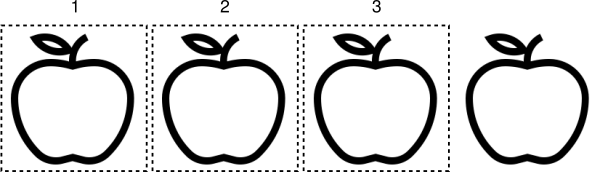
\includegraphics[scale=0.5]{figures/apples_counting.png}
\captionof{figure}{Counting}\label{fig:counting}
\end{figure}

According to the general counting principles, counting is devised to be what we see in \figref{fig:counting}. However, one could easily imagine an operation where, e.g., assigning a number to less than a whole entity or summing up complementary parts of corresponding entities to make up what counts as one is not prohibited. For instance, consider a quantificational operation that satisfies the general counting principle of non-overlap, but violates the principle of integrity. To illustrate this, let us assume illegal counting as depicted in \figref{fig:illegal-counting}.

\begin{figure}[h!]
\centering
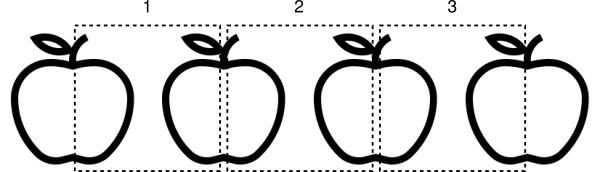
\includegraphics[scale=0.5]{figures/apples_not-counting.png}
\captionof{figure}{Illegal counting}\label{fig:illegal-counting}
\end{figure}

In contrast to \figref{fig:counting}, in this case numbers are associated with arbitrary sums of parts of distinct entities. Notice that those sums can be guaranteed to cover the total volume of all the relevant apples. If this were somehow ensured, in the discussed scenario we could obtain the same number as in \figref{fig:counting}. However, intuitively this operation is very different from counting. It is simply not what we do when we count.

Though the procedure illustrated in \figref{fig:illegal-counting} is not counting, it does not mean that it does not represent another quantificational operation human beings utilize for different purposes. In the next paragraphs, I will discuss what I believe to be the crucial difference between counting and measuring.

\subsection{Counting vs. measuring}\label{sec:counting-vs-measuring}

Intuitively, the difference between counting and measuring relies essentially on the fact that the former is about specifying how many objects of a certain kind there are in a particular context, whereas the latter concerns determining the quantity of a particular substance in relevant measure units. In principle, there are three possible views on the relationship between the two operations in question. The first one reduces measuring to a particular type of counting \citep[e.g.,][]{gil2013numeral}. The intuition behind such an approach is that measure words individuate in terms of quantity \citep{lyons1977semantics}. Consequently, instead of quantification over objects measuring is about counting units determined by measure words. An opposing approach is to view counting as a form of measuring. In particular, counting can be understood as measuring a quantity of an object in terms of natural units \citep{krifka1989nominal,krifka1995common}. Finally, the third option is to postulate that counting and measuring are two independent operations \citep{rothstein2017semantics}. In this study, I adopt the third perspective and present novel evidence in its favor. In particular, I propose that the distinction between counting and measuring can be reformulated in terms of quantificational principles introduced in the previous section. Though both counting and measuring obey the principle of non-overlap and maximality, only the former satisfies the principle of integrity. Measured quantities of a substance cannot overlap in order to ensure that things are not measured twice. Furthermore, a unit of measurement needs to correspond to the maximal quantity of matter to guarantee that measuring is exhaustive. However, only counting is sensitive to the topological make-up of entities it applies to.

To better understand the essence of the distinction, let us consider the following two scenarios. In the first scenario, illustrated in  \figref{fig:measuring-and-integrity}, someone has spilled some liquid on the table in such a way that there are two separate blobs $a$ and $b$ whose volume is one and a half milliliters each. In the second scenario, see \figref{fig:counting-and-integrity}, someone has simply put two cubes $c$ and $d$ on the table. Let us also assume that apart from the liquid and the cubes there is nothing else on the table in each of the cases, respectively.

\begin{figure}[h!]
	\centering
	\begin{tikzpicture}
	\coordinate (a) at (1.0,0.0);
	\coordinate (b) at (5.0,0.0);
	\draw[rounded corners=1mm] (a) \irregularcircle{1cm}{1mm};
	\draw[rounded corners=1mm] (b) \irregularcircle{1cm}{1mm};
	\node at (1.0,0.0) {$a$};
	\node at (5.0,0.0) {$b$};
	\end{tikzpicture}
	\caption{Measuring and integrity}
	\label{fig:measuring-and-integrity}
\end{figure}

\begin{figure}[h!]
	\centering
	\begin{tikzpicture}
	\draw (2.0,0.0) -- (4.0,0.0) -- (4.0,2.0) -- (2.0,2.0) -- (2.0,0.0);
	\draw (6.0,0.0) -- (8.0,0.0) -- (8.0,2.0) -- (6.0,2.0) -- (6.0,0.0);
	\node at (3.0,1.0) {$c$};
	\node at (7.0,1.0) {$d$};
	\end{tikzpicture}
	\caption{Counting and integrity}
	\label{fig:counting-and-integrity}
\end{figure}

Now, let us examine the sentences in \ref{ex:measuring-integrity} and \ref{ex:counting-integrity} describing the situations depicted in Figures \ref{fig:measuring-and-integrity} and \ref{fig:counting-and-integrity}, respectively. The statement in \ref{ex:measuring-integrity} is true despite the fact that one of the three milliliters must be split between a portion of $a$ and a portion of $b$ since each of the blobs consists of one and a half milliliters of liquid. On the other hand, \ref{ex:counting-integrity} is simply false. This contrast shows that units of measurement such as milliliters are not objects. In other words, unlike counting measuring does not care about individuation in terms of integrity and it indeed appears to be a distinct operation.

\ex. English (Guy Tabachnick, p.c.)\label{ex:measuring-counting-integrity}
\a. There are three milliliters of liquid on the table.\label{ex:measuring-integrity}
\b. \#There are three objects on the table.\label{ex:counting-integrity}

I argue that this is because counting is topology-sensitive whereas measuring is not. In other words, in measuring, units of measurement are not required to be assigned only to contiguous entities. There are multiple ways in which one could assign particular milliliters $u_1$, $u_2$, and $u_3$ to particular portions of $a$ and $b$, and \figref{fig:measuring-in-units} illustrates one possible distribution, with $u_2$ corresponding to the volume of liquid of a sum of one-third of $a$ and one-third of $b$. As long as the total volume of $a$ and $b$ equals three milliliters, \ref{ex:measuring-integrity} is true with respect to \figref{fig:measuring-and-integrity}.

\vfill
\begin{figure}[H]
	\centering
	\begin{tikzpicture}
	\coordinate (a) at (1.0,0.0);
	\coordinate (b) at (5.0,0.0);
	\draw[rounded corners=1mm] (a) \irregularcircle{1cm}{1mm};
	\draw[rounded corners=1mm] (b) \irregularcircle{1cm}{1mm};
	\draw[dashed] (1.29,-0.9) -- (1.29,0.9);
	\draw[dashed] (4.7,-0.9) -- (4.7,0.9);
	\node at (0.66,0.0) {$u_1$};
	\node at (3.0,0.0) {$u_2$};
	\node at (5.33,0.0) {$u_3$};
	\end{tikzpicture}
	\caption{Measuring in units}
	\label{fig:measuring-in-units}
\end{figure}
\vfill\pagebreak

Unlike measuring, counting is sensitive to what kind of topological structure entities in its domain have. In parallel to \figref{fig:measuring-in-units}, one could imagine that two-thirds of $c$ correspond to an object $o_1$, one-third of $c$ plus one-third of $d$ make up $o_2$, and the remaining two-thirds of $d$ correspond to $o_3$, as depicted in \figref{fig:counting-objects}. However, this is not how counting typically works. The statement in \ref{ex:counting-integrity} is false with respect to \figref{fig:counting-and-integrity} because counting assigns numbers to integrated individuated entities rather than arbitrary portions thereof.

\begin{figure}[h!]
	\centering
	\begin{tikzpicture}
	\draw (2.0,0.0) -- (4.0,0.0) -- (4.0,2.0) -- (2.0,2.0) -- (2.0,0.0);
	\draw (6.0,0.0) -- (8.0,0.0) -- (8.0,2.0) -- (6.0,2.0) -- (6.0,0.0);
	\draw[dashed] (3.33,0.0) -- (3.33,2.0);
	\draw[dashed] (6.66,0.0) -- (6.66,2.0);
	\node at (2.66,1.0) {$o_1$};
	\node at (5.0,1.0) {$o_2$};
	\node at (7.32,1.0) {$o_3$};
	\end{tikzpicture}
	\caption{Counting objects}
	\label{fig:counting-objects}
\end{figure}

I argue that what the contrast between truth-conditions of \ref{ex:measuring-integrity} and \ref{ex:counting-integrity} discussed above shows is that counting and measuring are in fact two distinct semantic operations, as proposed by \citet{rothstein2017semantics}. The core difference between the two boils down to the fact that counting is topology-sensitive, whereas measuring is not. In other words, it is misleading to think of measuring in terms of counting measure units \citep[pace][]{gil2013numeral}. If it were, similarly to \figref{fig:counting-and-integrity}, we would expect \ref{ex:measuring-integrity} to be false with respect to \figref{fig:measuring-and-integrity}, contrary to fact. 

The distinction gets even more salient if we realize that many numeral phrases can get a measure interpretation.\footnote{See \citet[p. 3]{rothstein2017semantics} for extensive discussion of ambiguities of another sort, namely the alternation between individuating and content readings of container words such as \textit{glass of water}.} For instance, consider the contrast between the scenarios described in \ref{ex:cooking-counting} and \ref{ex:cooking-measuring}. In \ref{ex:cooking-counting-setup}, the numeral phrase \textit{three apples} denotes a plurality of integrated wholes, i.e., distinct individuated objects, and thus it can be felicitously continued by \ref{ex:cooking-counting-continuation}. In other words, since the referents of the phrase satisfy conditions specified by the general counting principles, they can be put in a one-to-one correspondence with numbers.  

\ex. English (Guy Tabachnick, p.c.)\\
	extit{Scenario}: John is cooking with his child. They put three whole apples on a table. John says:\label{ex:cooking-counting}
\a. There are three apples on the table\dots\label{ex:cooking-counting-setup}
\b. Let's count them together: one, two, three.\label{ex:cooking-counting-continuation}

On the other hand, the same phrase in the context of \ref{ex:cooking-measuring} gets a measure reading. Given that the slices in the bowl are placed in such a way that it is impossible to retrieve the original part-whole structures of individual apples, \textit{three apples} does not refer to distinct objects but rather to the volume corresponding to three apples. Consequently, it is distinctively odd to continue the sentence in \ref{ex:cooking-measuring-setup} with \ref{ex:cooking-measuring-continuation}. All things considered, \ref{ex:cooking-counting-setup} presumes an operation depicted in \figref{fig:counting}, whereas \ref{ex:cooking-measuring-setup} does not.

\ex. English (Guy Tabachnick, p.c.)\\
	extit{Scenario}: John is cooking with his child. They sliced three apples and put the slices into a bowl. John says:\label{ex:cooking-measuring}
\a. There are three apples in the bowl\dots\label{ex:cooking-measuring-setup}
\b. \# Let's count them together: one, two, three.\label{ex:cooking-measuring-continuation}

The contrasts discussed above prove that counting indicates integrity or at least easily retrievable traces of integrity of entities it applies to, whereas measuring ignores this factor. Though monotonic systems of measurement track part-whole relations \citep{schwarzschild2002grammar}, they do not seem to be sensitive to topological notions. On the other hand, counting does care about the spatial arrangement of parts making up wholes. This strongly suggests that the two operations in question are distinct from each other. Perhaps, one could argue that despite syntactic as well as semantic differences between numeral phrases and measure phrases \citep[see][]{rothstein2017semantics} counting is a very special case of measuring \citep[see][]{krifka1989nominal,krifka1995common}. In particular, measuring could be thought of as a more general quantificational procedure.  However, for the sake of what this study is about I will assume that measuring and counting are two distinct semantic operations. In the next section, I will propose how general counting principles extend to subatomic quantification.

\subsection{Subatomic quantification}\label{sec:subatomic-quantification}

In Chapters \ref{ch:partitives-and-part-whole-structures}, \ref{ch:exploring-topological-sensitivity}, and \ref{ch:multipliers}, we saw that there is substantial evidence showing that natural language semantics is sensitive to the fact that entities we refer to by means of nominal constructions consist of parts and that there are linguistic means to quantify over such parts. On the other hand, in the previous section I postulated the general counting principles of non-overlap, maximality, and integrity. So far, we have seen that there are good reasons to believe that these quantificational constraints capture what humans do when they count objects. In this section, I argue that the proposed set of rules constitutes a universal mechanism that can be applied not only to whole individuals but also when counting parts of objects. In other words, I posit that subatomic quantification is subject to the very same constraints as quantification over wholes.

Analogously to what we saw in \figref{fig:counting}, counting at the subatomic level presumes mereological maximality and topological integrity of entities subject to quantification. Typically, counting is sensitive to the fact that some parts are cognitively more salient within the part-whole structure of an object than others. This seems to correspond to what \citet{champollion_krifka2016mereology} call structured parthood as well as to the distinction between specific and arbitrary subdivisions of a whole into parts introduced in philosophical considerations, as already mentioned in Chapter \ref{ch:introduction} \citep[e.g.,][]{krecz1986parts,markosian1998brutal,jennings2010against}. Notice that what counts as a cognitively salient part can vary with respect to the context. For instance, consider the two sentences in \ref{ex:cognitively-salient-parts}. 

\ex. English (Guy Tabachnick, p.c.)\label{ex:cognitively-salient-parts}
\a. Both parts of the teddy bear are painted.\label{ex:cognitively-salient-parts-both}
\b. Two parts of the teddy bear are painted.\label{ex:cognitively-salient-parts-two}

Assume John's daughter has a teddy bear called Fuzzy Wuzzy. In a situation where she has covered Fuzzy Wuzzy's entire left half with red paint and its entire right half with black paint, John might want to say \ref{ex:cognitively-salient-parts-both}. In such a case, the total volume of matter making up the teddy bear is partitioned in such a way that the cognitively salient parts are its left half and its right half.\footnote{The sentence in \ref{ex:cognitively-salient-parts-both} appears to be slightly degraded due to the fact that instead of \textit{part} a more accurate partitive word, i.e., \textit{half}, could have been used. Many thanks to Guy Tabachnick for discussing the English examples with me.} On the other hand, in a scenario where John's daughter painted Fuzzy Wuzzy's left paw red and its right paw black, the count explicit partitive in \ref{ex:cognitively-salient-parts-two} refers to the teddy bear's body parts. Nevertheless, what cognitively salient parts have in common is that given a particular context they are disjoint. This brings us to the relevance of the principle of non-overlap in subatomic quantification.\largerpage

Since there are numerous ways in which one could divide an object into parts, there are multiple portions of matter of which the property of being part of that object holds. For instance, \figref{fig:overlapping-parts} illustrates a number of entities the phrase \textit{part of the apple} could refer to. Notice that none of them is disjoint from the others, i.e., all of them share a part with at least one other part. However, the principle of non-overlap states that such entities cannot be counted. Similarly to arbitrary portions of mass, e.g., juice, arbitrary parts of an apple avert individuation since they are not well-defined bounded integrated objects and it is virtually impossible to distinguish them from other parts. This means that not all parts are equal with respect to countability. Some of them are countable, whereas others are not. Crucially, only those divisions of a whole into parts can be enumerated that are perceived as involving only non-overlapping parts.

\begin{figure}[h!]
\centering
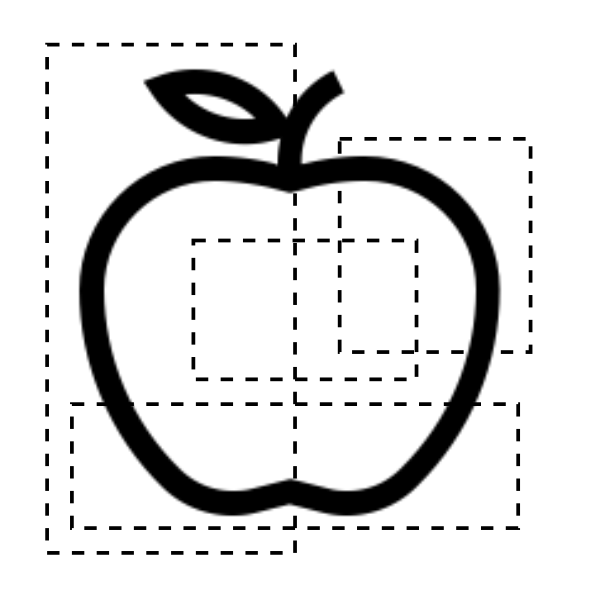
\includegraphics[scale=0.5]{figures/apple_overlap.png}
\captionof{figure}{Overlapping parts}\label{fig:overlapping-parts}
\end{figure}

Another issue concerns the principle of maximality. What counts as part of an object can also consist of smaller parts. Notice that such parts of parts also satisfy the property of being part of that object. However, the general counting principles require that only entities in their mereological entirety can be associated with a number. This means that once a particular division of an individual into parts has been executed in a given counting context, those parts are immutable and are treated as objects in their own right. Consequently, the principle of maximality applies as it would in a situation when one counts whole individuals. In other words, given a partition, non-overlapping parts are assumed to be maximal with respect to how the whole has been divided.

Finally, as we saw in the previous section, countability is also governed by the principle of integrity. However, as we saw in Chapter \ref{ch:exploring-topological-sensitivity}, extensions of expressions referring to parts of objects do not necessarily involve topological commitments, i.e., parts need not be continuous. For instance, let us consider explicit entity partitives. There is definitely a sense in which two or more separated portions of matter within an object are part of that object, and thus a topology-neutral explicit entity partitive construction would be true of such a configuration. Nevertheless, as any arbitrary sum such entity is not countable since associating it with a number would clearly violate the principle of integrity. Therefore, only sets including parts that are mereologically maximal integrated entities that do not overlap can be enumerated. In other words, only a subset of possible divisions of an object is fit for counting.

Having this in mind, let us see how the general counting principles apply in the context of subatomic quantification. For this purpose, let us assume John's daughter wants to count parts of her teddy bear Fuzzy Wuzzy. \figref{fig:counting-of-parts} represents an exemplary situation that intuitively fits what we expect from counting. 

\begin{figure}[h!]
\centering
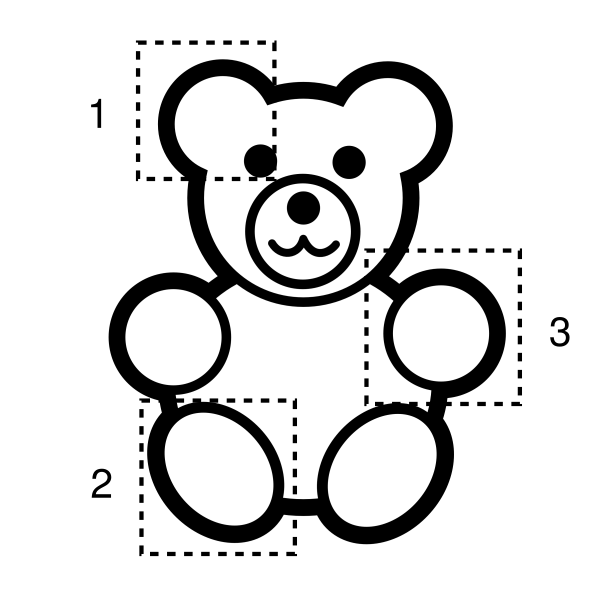
\includegraphics[scale=0.5]{figures/toy_counting-parts.png}
\captionof{figure}{Counting of parts}\label{fig:counting-of-parts}
\end{figure}

The operation illustrated above assigns numbers to cognitively salient non-overlapping parts of Fuzzy Wuzzy, namely its ear, leg, and paw. Those parts constitute mereologically maximal and integrated entities, i.e., though they are elements of a larger whole, when counted they are treated as objects in their own right. This means that, e.g., number 1 is associated with Fuzzy Wuzzy's whole ear and there is no part of that ear that is left out. Also, an ear is a continuous part that comes in one piece. To sum up, since the depicted division of the teddy bear consists of elements that are disjoint, maximal, and integrated, all the counting principles are satisfied and the set of parts can be enumerated.

On the other hand, one could imagine another operation, e.g., one such as that illustrated in \figref{fig:illegal-counting-of-parts}. Though it is definitely logically possible, it seems weird and would intuitively be rejected as counting. There are two reasons why this is so. The first reason is that the indicated ear and leg do not constitute a continuous integrated part that would be cognitively salient. Therefore, assigning them the number 1 violates the principle of integrity. In other words, there is a sense in which an ear and a leg are part of the teddy bear, but they are not \textit{a part} of it and only entities that can be considered as such can satisfy the countability condition. The second reason is that the marked paw is not disjoint with the right half of the teddy bear which of course violates the principle of non-overlap. Given the division in \figref{fig:illegal-counting-of-parts}, the paw in question would be counted twice and since counting requires that an entity can be associated with a number once and once only, the depicted operation fails to satisfy the general counting principles and represents what I call illegal counting at the subatomic level, recall \figref{fig:illegal-counting}.

\begin{figure}[h!]
\centering
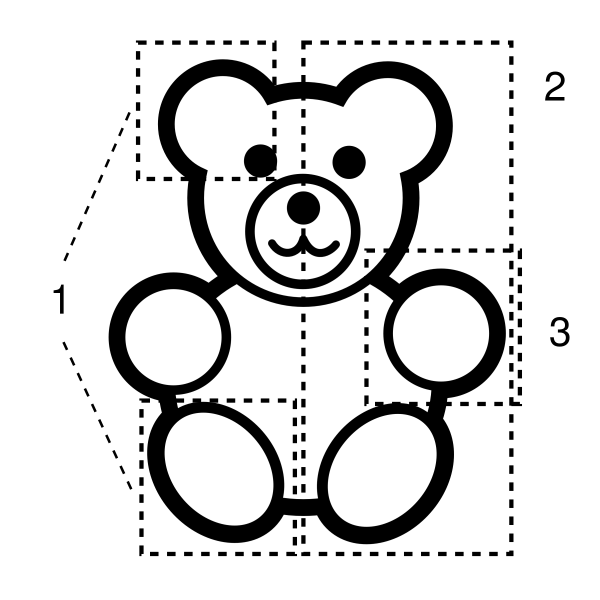
\includegraphics[scale=0.5]{figures/toy_not-counting-parts.png}
\captionof{figure}{Illegal counting of parts}\label{fig:illegal-counting-of-parts}
\end{figure}

All things considered, counting at the subatomic level presumes assigning numbers to salient parts of a whole constituting disjoint integrated entities that are maximal with respect to a given partition. In other words, once it is decided what counts as a part, it is treated as an individuated object in its own right and all discussed constraints concerning counting apply. The key conclusion is that there is one universal mechanism governing quantification over wholes as well as subatomic quantification, and exploring the latter can reveal some fundamental properties of countability in general that otherwise might be difficult to recognize.

\section{Summary}\label{sec:summary-ch5}

In this chapter, I provided a general conceptual framework that will serve as a basis for developing a formal account for subatomic quantification in natural language. I suggested how the linguistic evidence presented in Chapters \ref{ch:partitives-and-part-whole-structures}, \ref{ch:exploring-topological-sensitivity}, and \ref{ch:multipliers} correlates with findings in cognitive psychology. In particular, in the first part of the chapter I reviewed several representative studies in the research indicating the following. First, there is compelling evidence that humans possess an innate ability to perceptually distinguish between objects, i.e., bounded integrated entities, and substances, i.e., shapeless scattered portions of matter, and that this contrast correlates with the mass/count distinction in grammar, though the correspondence is imperfect. Specifically, integrated solid things are predictably referred to by count nouns, but there is a class of mass terms that also refer to objects. Importantly, the object/mass distinction is not based on ontological properties of entities in some objective sense but rather it is construed by human cognition. Second, the ability to simultaneously perceive parts as elements of a whole and a whole as a collection of parts manifests itself in early childhood. The capacity to intuitively distinguish between parts and wholes guides vocabulary acquisition. Finally, human number sense appears to be sensitive to whether counted items are conceptualized as integrated objects. Experimental evidence shows that young children always count each separate physical entity as one. Even if they are instructed to do otherwise or given clues that two elements might be considered one broken thing, they ignore them and simply cannot avoid counting contiguous entities. This suggests that further development of quantification in older humans rests on a mechanism  individuating singular objects in terms of spatial integrity.

In the second part of this chapter, I presented the three claims that constitute the conceptual core of this study. I postulated that natural language is sensitive to how the spatial relationship holding between parts of a particular entity is conceptualized. The relevance of the topological notion of integrity manifests itself primarily in how the nominal lexicon is classified into different grammatical categories. In particular, count singular nouns prototypically designate integrated wholes, i.e., encode information concerning a particular spatial configuration of parts their referents consist of, whereas plurals denote arbitrary sums thereof, i.e., presuppose integrated wholes as parts but impose no topological constraints on them.

The second claim regards what I call the general counting principles. I posit that counting is a special kind of quantificational operation that presumes certain properties of entities that are put in a one-to-one correspondence with numbers. Specifically, the principle of non-overlap guarantees that enumerated entities are disjoint, and thus no thing is counted twice. On the other hand, the principle of maximality requires that numbers are associated with entities in their mereological entirety, i.e., no part is left out. Finally, the principle of integrity ensures that what can be counted needs to be conceptualized as something that comes in one piece. This constraint excludes arbitrary sums of individuals as well as scattered entities such as substances. Altogether, the general counting principles guarantee that sets that can be enumerated consist only of elements that are discrete object.

The final claim extends the general counting principles to subatomic quantification. In other words, I postulate the quantificational mechanism described above is a universal mechanism that can apply both at the level of wholes and at the level of parts. In the next chapter, I will introduce a theory of wholes called mereotopology in which the formal account for subatomic quantification will be grounded. In particular, it will enable us to capture various subtle topological distinctions including the intuitive notion of an integrated whole as opposed to an arbitrary sum of parts. This will provide means to model not only the fact that some entity is part of something else but also how individual parts are spatially arranged within a whole configuration.
